% Standard template book
\documentclass[11pt, a4paper, oneside]{book}

%%%%%%%%%%%%%%%%%%%%%%%%%%%%%
% Packages
%%%%%%%%%%%%%%%%%%%%%%%%%%%%%

% Better looking urls
\usepackage[hyphens]{url}

% During testing to se all the margins
% \usepackage[showframe]{geometry}
% Package parskip is supposed to fix whitespaces in list
% and other environments when you alter the \parskip setting.
% https://en.wikibooks.org/wiki/LaTeX/Paragraph_Formatting
\usepackage{parskip}

% Remove indentation of first line in each paragraph
\setlength{\parindent}{0cm} % Default is 15pt.

% Add whitespace between paragraphs
\setlength{\parskip}{3mm plus4mm minus3mm}

% Alter headers and footers
\usepackage[pagestyles]{titlesec}
\newpagestyle{footerPageNumberMiddle}{\setfoot[\thepage][][]{}{\thepage}{}}

% Adding \figure support
\usepackage{graphicx}

% Source code support
\usepackage{listings}

% Math support
\usepackage{amsmath} % Math
\usepackage{amsthm} % Theorems and proofs

% Theorems details
% http://www.sharelatex.com/learn/Theorems_and_proofs
\theoremstyle{definition}
\newtheorem{defi}{Definition}
\newtheorem{theorem}{Theorem}[section]
\newtheorem{lemma}[theorem]{Lemma}

% Change whitespace above theorems
\makeatletter
\def\thm@space@setup{%
    \thm@preskip=10pt \thm@postskip=0pt
}
\makeatother

% Add support for list of abbreviations
\usepackage{nomencl}
\makenomenclature
\setlength\nomlabelwidth{3cm} % Change this value to align the list of abbrev.

% Caption support in figures
% with sub-figures
\usepackage[hypcap=true]{caption}
\usepackage[hypcap=true,list=true,listformat=simple]{subcaption}

% Add links within the PDF
% All links are turned into booksmarks as well
\usepackage[bookmarks, hidelinks]{hyperref}

% Make sure hyperlinks to figures link to top of image
% and not to the caption.
\usepackage[all]{hypcap}

% Make it possible to add bookmarks without entries in the
% table of content.
\usepackage{bookmark}


%%%%%%%%%%%%%%%%%%%%%%%%%%%%%
% Document start and frontmatter
%%%%%%%%%%%%%%%%%%%%%%%%%%%%%
\begin{document}
\frontmatter

% Title
\title{Master thesis - Notes about references}

% Author
\author{Christoffer Holmstedt}

\maketitle

%%%%%%%%%%%%%%%%%%%%%%%%%%%%%
% Abstract
%%%%%%%%%%%%%%%%%%%%%%%%%%%%%

\cleardoublepage
\pdfbookmark{Abstract}{Abstract}
\chapter*{Abstract}
\thispagestyle{empty} % No page numbering on this page
Space Plug-and-Play Architecture (SPA) is a set of standards to make it easier
to build small satellites. Focus is put on improving the integration phase and
the time consuming validation and verification process by introducing
plug-and-play functionality. From mission call-up to operational satellite it
should only take six days.

A SPA network consists of several different types of subnets with different
pros and cons. For each processing node there must be one Local Subnet Manager
(SM-L). The SM-L can communicate over different communication protocols
depending on how the respective local subnet is set up, one option is UDP/IP.

In this thesis Ada Protected Objects is presented as a viable option for
inter-process communication instead of UDP/IP in a SPA network. This thesis
present the initial work towards a SPA Local Subnet Adaptation that builds on
language constructs in Ada such as Ada Tasks and Protected Objects.  The system
design and implementation is verified deadlock free with UPPAAL but shows
indications of livelock possibilities. The severity of these livelock
situations is discussed in the conclusion.

% Keywords
\textbf{Keywords:} Space plug-and-play Architecture, SPA, UPPAAL, Timed
automata, Ada, Ravenscar, Unified Common Architecture, UNICA, Virtual Network
Protocol, VNP


%%%%%%%%%%%%%%%%%%%%%%%%%%%%%
% Acknowledgement
%%%%%%%%%%%%%%%%%%%%%%%%%%%%%

\cleardoublepage
\pdfbookmark{Acknowledgement}{Acknowledgement}
\chapter*{Acknowledgement}
\thispagestyle{empty} % No page numbering on this page
TODO


%%%%%%%%%%%%%%%%%%%%%%%%%%%%%
% Table of Content, List of Figures/Tables
%%%%%%%%%%%%%%%%%%%%%%%%%%%%%

\cleardoublepage
\pdfbookmark{\contentsname}{Contents}
\tableofcontents

\listoffigures
\addcontentsline{toc}{chapter}{\listfigurename}
\listoftables
\addcontentsline{toc}{chapter}{\listtablename}

% List of Abbrevations
% To align the columns change the value further up in this file next
% to loading the nomencl package.
\renewcommand{\nomname}{List of Abbreviations}
\cleardoublepage%
\printnomenclature
\addcontentsline{toc}{chapter}{\nomname}

%%%%%%%%%%%%%%%%%%%%%%%%%%%%%
% Mainmatter - The Report
%%%%%%%%%%%%%%%%%%%%%%%%%%%%%

\mainmatter
\pagestyle{footerPageNumberMiddle}
\chapter{Ada Programming Language}

\section{Guide for the use of the Ada programming language in high integrity
systems}

\subsection{Facts}
\begin{description}
    \item[Label:] web:ada-high-integrity \cite{web:ada-high-integrity}
    \item[Year:] XXXX
\end{description}

\subsection{Notes and important findings}
Aenean luctus quam ut neque viverra, quis vulputate mi hendrerit. Nunc id leo

\subsection{Thoughts and ideas}
Phasellus nec erat vehicula, ornare urna sit amet, dictum metus. Duis ac

\subsection{Related references}
\begin{itemize}
    \item Item one.
\end{itemize}

\chapter{Space Plug-and-Play Architecture}\label{ch:spa}
Space plug-and-play Architecture (SPA) is a set of standards that define how
different players can create plug-and-play components that can easily be
assembled to form a complete satellite for a specific mission. The standards
are published by American Institute of Aeronatuics and Astronautics (AIAA). The
standards range from how power supply should be handled to how components
communicate in the application layer, focus in this report is put on the
software parts.

To describe how a SPA network works some terminology needs to be defined. All
nodes in a SPA network are called "components", there is no differentiation
between software and hardware components. Each component has a "Component
Universally Unique Identifier" (CUUID) which is 128 bit long. Each component
also has an "Extensible Transducer Electronic Data Sheet" (xTEDS) file that
describes respective components capabilities. To be able to support different
underlying link layer technologies such as Ethernet, Spacewire and one-wire
(I2C), most functionality has been put in the application layer. This means
that a SPA network can be built with any combination of link layer "subnets",
for example a SPA network can consist of two Spacewire subnets and one Ethernet
subnet.

\nomenclature{\textbf{CUUID}}{\textbf{Component Universally Unique Identifier}}

The important concepts to remember is that each SPA component is
connected to one or more SPA subnets, on each SPA subnet there is a subnet
manager (SM-x) that acts as a gateway to other SPA subnets and when SPA subnets
are linked together they form a SPA network. To make things clear, a single SPA
subnet with a CAS, LS and SM-x is also a SPA network.

Another SPA subnet is the SPA Local Subnet. Each processing node that can
have multiple SPA components running on it has a "SPA Local Subnet Manager"
(SM-L).  Components within a processing node should do inter-process
communication over UDP/IP \cite{spa:local-subnet}.

Components communicate with each other with the help of "logical addresses"
that each component recieves during boot up. It is the responsiblity of the
"Central Addressing Service" (CAS) to hand out logical addresses to all
components in the SPA network through the connected Subnet Managers. After a
component receives its logical address it can share its xTEDS file with other
components. It is the responsibility of the "Lookup Service" to keep track of
the capabilities of each component in the SPA network.

To describe what a SPA network can look like figure
\ref{fig:minimal_spa_network} shows a minimal SPA network which consists of a
CAS, LS, a sensor and a monitor application, all running on the same processing
node and in the same local subnet managed by the SM-L.

\begin{figure}[h]
    \centering
    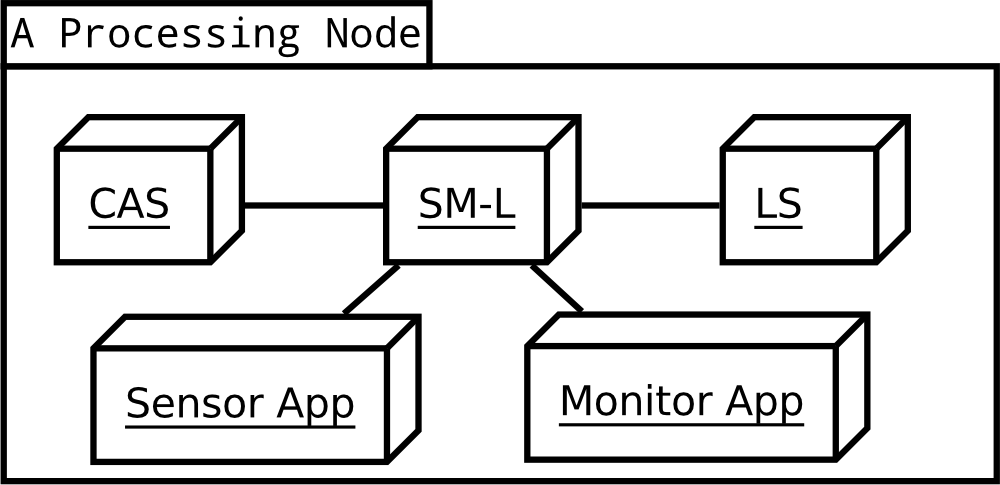
\includegraphics[width=\textwidth]{figures/minimal_spa_network}
    \caption{A processing node running a minimal SPA network.}
    \label{fig:minimal_spa_network}
\end{figure}

A more complex SPA network is shown in figure \ref{fig:complex_spa_network}.
Three different processing nodes are connceted to each other over a
SPA-Ethernet subnet. The CAS, LS and Monitor Application are now running on
different nodes and the sensor application is located on its own embedded
device.

\begin{figure}[h]
    \centering
    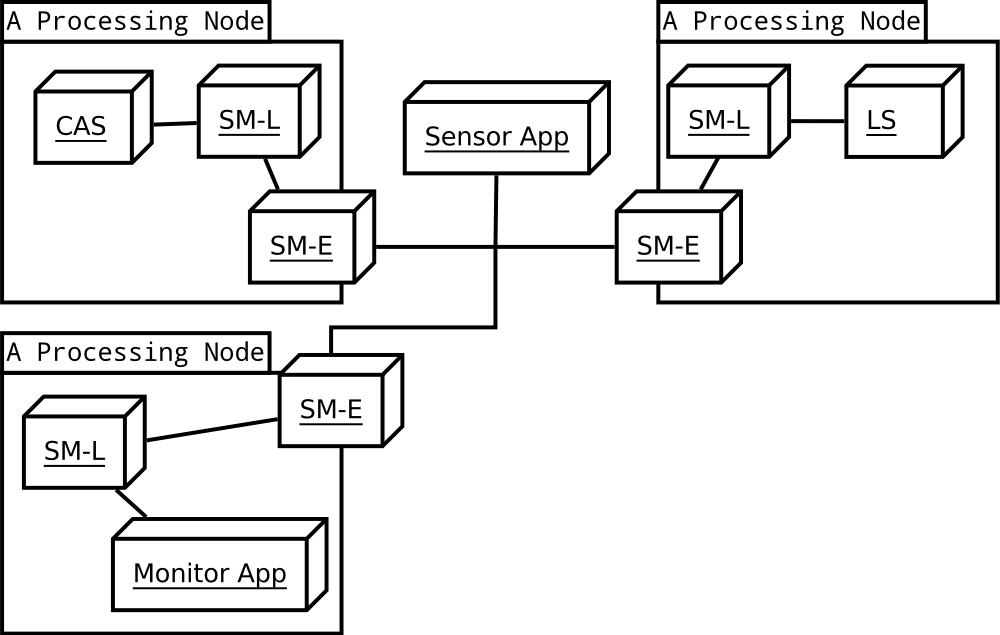
\includegraphics[width=\textwidth]{figures/complex_spa_network}
    \caption{A SPA network with multiple subnets.}
    \label{fig:complex_spa_network}
\end{figure}

For a detailed view on how SPA works the SPA standards is the best source for
information. The SPA standards and drafts that specify software requirements
are the Logical Interface standard \cite{spa:logical-interface}, Networking
standard \cite{spa:networking}, Local Subnet Draft \cite{spa:local-subnet},
Ontology Standard \cite{spa:ontology} and System Capabilities Standard
\cite{spa:system-capabilities}.


% \section{Virtual Network and the Virtual Network Protocol}
% TODO: Finish of with the definition of Virtual Network, Virtual Network
% Protocol and how it relates to SPA.
%
% TODO: Is this needed or should VNP perhaps only be mentioned in context with
% development efforts and code? This would mean that all comments about VN/VNP is
% pushed to the results and conclusion parts...perhaps some in the method.

\chapter{Ada Programming Language}

\section{Guide for the use of the Ada programming language in high integrity
systems}

\subsection{Facts}
\begin{description}
    \item[Label:] web:ada-high-integrity \cite{web:ada-high-integrity}
    \item[Year:] XXXX
\end{description}

\subsection{Notes and important findings}
Aenean luctus quam ut neque viverra, quis vulputate mi hendrerit. Nunc id leo

\subsection{Thoughts and ideas}
Phasellus nec erat vehicula, ornare urna sit amet, dictum metus. Duis ac

\subsection{Related references}
\begin{itemize}
    \item Item one.
\end{itemize}

\chapter{Design with UML and UPPAAL}

%%%%%%%%%%%%%%%%%%%%%%%%%%%%%%%%%%%%%%%%%%%%%%%%%%%%%%%%%%%%%%%%%
% Analyzing the Redesign of a Distributed Lift System in UPPAAL
%%%%%%%%%%%%%%%%%%%%%%%%%%%%%%%%%%%%%%%%%%%%%%%%%%%%%%%%%%%%%%%%%
\section{Analyzing the Redesign of a Distributed Lift System in UPPAAL}

A well explained case study about a lift system with a CAN bus modeled in
UPPAAL to detect some liveness and safety issues. This report might have some
valuable references but it's already 10 years old.

\begin{description}
    \item[Label:] pang2003 \cite{pang2003}
    \item[Year:] 2003
    \item[Abbrevations and terms:] None.
\end{description}

\begin{itemize}
    \item No specifc comments.
\end{itemize}

%%%%%%%%%%%%%%%%%%%%%%%%%%%%%%%%%%%%%%%%%%%%%%%%%%%%%%%%%%%%%%%%
% Object-Oriented Systems Analysis and Design: Using UML
%%%%%%%%%%%%%%%%%%%%%%%%%%%%%%%%%%%%%%%%%%%%%%%%%%%%%%%%%%%%%%%%
\section{Object-Oriented Systems Analysis and Design: Using UML}
A good book which gave me a crash course in UML or rather repitition on which
diagrams to use when and why. A few good examples in the book, didn't read the
case-studies.

\begin{description}
    \item[Label:] book:bennett2010 \cite{book:bennett2010}
    \item[Date:] 2010
    \item[Abbrevations and terms:]
        UML,\nomenclature{\textbf{UML}}{\textbf{Unified Modeling Language}}
        USDP,\nomenclature{\textbf{USDP}}{\textbf{Unified Software Development
        Process}}
\end{description}


\begin{itemize}
    \item Page 118, UML has two types of diagrams, structural and behavioural.
    \item Page 120, This page shows icons for package, subsystem and model.
    \item Page 123, section 5.3.2, Activity diagrams.
    \item Page 127, mentions "activity partitions" and its old name
        "swimlanes".
    \item Page 129, fig 5.15, Figure of the USDP (Unified Software Development
        Process).
    \item Page 141, section 6.2.2, three types of requirements: functional,
        non-functional and usability.
    \item Page 157-158, mentions difference between <<extend>> and <<include>>.
    \item Page 198-201, section 7.5.2, interesting section about boundary,
        entity and control stereotypes.
    \item Page 236-237, section 8.2.3, mentions generalization, encapsulation
        and information hiding. Short paragraph about compoisition.
    \item Page 242, section 8.3.2, composition in detail.
    \item Page 248-251, section 8.4.2, components in detail.
    \item Page 263, Figure 9.3, great sequence diagram example.
    \item Page 264, section 9.3.1, describes how frames are used e.g. in a
        sequence diagram (sd).
    \item Page 278, section 9.3.7, difference between active and passive
        objects in sequence digrams.
    \item Page 279, list of sequence digram's "integration operators" e.g. alt,
        opt and loop.
    \item Page 286, section 9.6, timing diagrams, related to state machines
        (chapter 11).
    \item Page 292, chapter 10. How to specify operations with pre/post
        condtions and contracts.
    \item Page 354, section 12.5.1, list of qualities (quality attributes(?))
        with descriptions.
    \item Page 422, chapter 15 about Design patterns goes through singleton and
        composite.
\end{itemize}

%%%%%%%%%%%%%%%%%%%%%%%%%%%%%%%%%%%%%%%%%%%%%%%%%%%%%%%%%%%%%%%%%%%%%
% A Ravenscar-Compliant Run-Time Kernel for Safety Critical Systems
%%%%%%%%%%%%%%%%%%%%%%%%%%%%%%%%%%%%%%%%%%%%%%%%%%%%%%%%%%%%%%%%%%%%%
\section{A Ravenscar-Compliant Run-Time Kernel for Safety Critical Systems}
A good walkthrough about how a "naked" Run-Time Kernel is verified with UPPAAL.
Includes a good collection of references on Model-checking with automatons.

\begin{description}
    \item[Label:] lundqvist2003 \cite{lundqvist2003}
    \item[Date:] 2003
    \item[Abbrevations and terms:] None.
\end{description}

\begin{itemize}
    \item Page 8, section 4, some interesting references about timed automata
        and model-checking.
\end{itemize}

%%%%%%%%%%%%%%%%%%%%%%%%%%%%%%%%%%%%%%%%%%%%%%%%%%%%%%%%%%%%%%%%%%%%%
% Developing UPPAAL over 15 years
%%%%%%%%%%%%%%%%%%%%%%%%%%%%%%%%%%%%%%%%%%%%%%%%%%%%%%%%%%%%%%%%%%%%%
\section{Developing UPPAAL over 15 years}
Interesting paper about UPPAAL but not much value for my master thesis.

\begin{description}
    \item[Label:] behrmann2011 \cite{behrmann2011}
    \item[Date:] 2011
    \item[Abbrevations and terms:] None.
\end{description}

\begin{itemize}
    \item Page 5/137, first rule of survival "one should have a solid design
        and stick with it".
    \item Page 6/138, section "Tool building process", doxygen for comments,
        that's it.
    \item Page 6/138, intersting idea to use binary search to detect which
        addition of functionality introduced a newly detected bug.
    \item Page 7/139, Yahoo group for community communication.
\end{itemize}

%%%%%%%%%%%%%%%%%%%%%%%%%%%%%%%%%%%%%%%%%%%%%%%%%%%%%%%%%%%%%%%%%%%%%%
% Model Checking Applied to Embedded Software of University Satellite
%%%%%%%%%%%%%%%%%%%%%%%%%%%%%%%%%%%%%%%%%%%%%%%%%%%%%%%%%%%%%%%%%%%%%%
\section{Model Checking Applied to Embedded Software of University Satellite}

A good report with the basis in a master thesis about how to properly do
model-checking and why. This reports checks that the design of the system
works as intended and no deadlocks can occur. With the help of model-checking
some problems with the requirements specification were dedicted and fixed.

\begin{description}
    \item[Label:] alencar2013 \cite{alencar2013}
    \item[Year:] 2013
    \item[Abbrevations and terms:] None.
\end{description}

\begin{itemize}
    \item Page 2/127, section 2, good reasoning and listing of references.
\end{itemize}

%%%%%%%%%%%%%%%%%%%%%%%%%%%%%%%%%%%%%%%%%%%%%%%%
% New reference
%%%%%%%%%%%%%%%%%%%%%%%%%%%%%%%%%%%%%%%%%%%%%%%%
%\section{Title}
%
% Some thoughts about the reference here.
%
%\begin{description}
%    \item[Label:] web:ada-high-integrity \cite{web:ada-high-integrity}
%    \item[Date:] MM-YYYY
%    \item[Abbrevations and terms:]
%       ASIS,\nomenclature{\textbf{ASIS}}{\textbf{Ada Semantic Interface
%       Specification} provides a standard mechanism for obtaining information
%       about an Ada program or its components. ASIS is an ISO standard.}
%\end{description}
%
%
% \begin{itemize}
%     \item Page 34, section 5.11 has valuable information about access types and
%     \item Page 35, good reasoning about the use of exceptions.
%     \item Page 37, section 5.13 has some good notes on Tasking in
% \end{itemize}


%%%%%%%%%%%%%%%%%%%%%%%%%%%%%
% Appendix
%%%%%%%%%%%%%%%%%%%%%%%%%%%%%

\bibliographystyle{plain}
\bibliography{../references}  % references.bib is the file with all references. 
\addcontentsline{toc}{chapter}{\bibname}

\appendix
% \chapter{LaTeX examples}

\section{Example of abbrevations}
This is a short example of abbreviations are added to the list of abbrevations.
The term Fig.\nomenclature{Fig.}{Figure} is now in the List of abbrevations.
The term Img.\nomenclature{Img.}{Image} is now in the List of abbrevations.
The term Tab.\nomenclature{Tab.}{Table} is now in the List of abbrevations.
The term Long Name.\nomenclature{Long Name Long Name}{This is an example of a long
abbrevation that has an even longer description that will hopefully span at
least two rows.} is now in the List of abbrevations.


\section{Figures and images}
Lorem ipsum dolor sit amet, consectetur adipiscing elit. Sed nec ligula vel
ante placerat dapibus. Vestibulum non sollicitudin tellus. Sed varius
vestibulum libero, in euismod purus dapibus sed. Pellentesque malesuada, urna
nec lobortis egestas, felis elit varius ante, in tincidunt nunc metus id diam.
Morbi sagittis velit at ipsum sodales, in tempor nulla volutpat. Integer a
neque eros. In ipsum erat, pellentesque at dapibus eget, pretium sed risus.
Vivamus quis metus vitae felis tempus vulputate eget id lacus. Aenean sit amet
gravida quam, et ornare erat. Praesent ullamcorper mattis dolor, non interdum
orci aliquam a. In tincidunt semper lectus. Duis quis mi ac felis vehicula
mollis. Fusce molestie arcu urna, a tempor turpis mattis nec. Aenean in massa a
risus euismod aliquet vel non libero.

\subsection{One figure}

\begin{figure}[h]
    \centering
    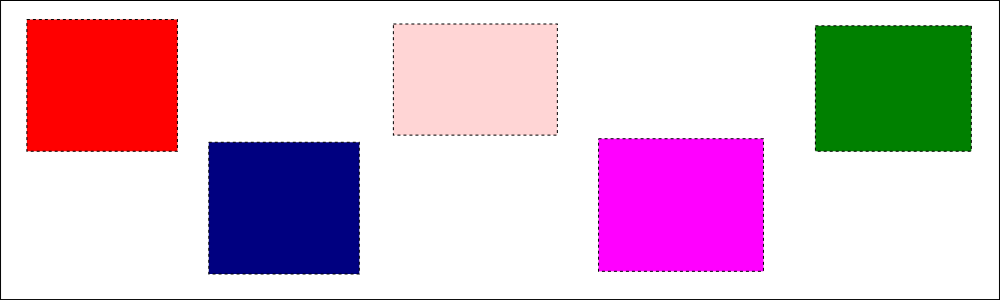
\includegraphics[width=\textwidth]{figures/test_image}
    \caption{Test Image}
    \label{fig:test_image}
\end{figure}

Aenean luctus quam ut neque viverra, quis vulputate mi hendrerit. Nunc id leo
id dui semper blandit. Nulla orci ligula, posuere non lacinia non, aliquet non
massa. Quisque gravida in mi eget volutpat. Fusce convallis felis sed dolor
ornare rhoncus. Nullam sed lacus id lectus venenatis pulvinar eget ac arcu. Sed
id turpis in leo sollicitudin euismod nec ac enim. Nunc vitae lacus lectus.
Class aptent taciti sociosqu ad litora torquent per conubia nostra, per
inceptos himenaeos. Figure \ref{fig:test_image}, Integer gravida, orci vitae
viverra ullamcorper, quam libero tempor est, non gravida magna eros id augue.
In lobortis et est auctor congue. Aliquam sed ante lacus. Vestibulum aliquam
elit eget elementum facilisis. Quisque eget felis eu leo pharetra pharetra.

\subsection{Two sub-figures}
Nulla at purus volutpat, accumsan arcu eget, commodo felis. Cras consequat
risus at rhoncus pellentesque. Aliquam tempor sodales purus in sodales. Sed ut
augue lobortis, mattis felis a, ultricies ante. Pellentesque ac tristique
ipsum, aliquet fermentum ipsum. Sed vel elit sed odio vestibulum semper id eget
enim. Nulla sed hendrerit tortor. Aliquam quam nisl, tempor ut nisl vel,
tristique facilisis libero. Suspendisse id rutrum ante. Duis sed luctus sapien.
Nullam sed quam justo.
\begin{figure}[h]
    \begin{subfigure}[b]{0.5\linewidth}
        \centering
            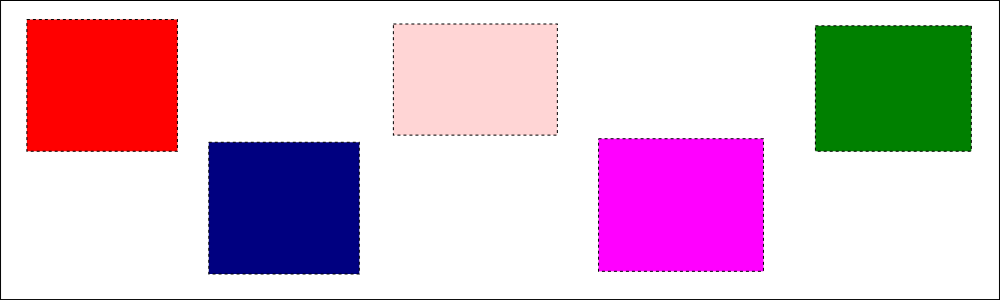
\includegraphics[width=0.9\textwidth]{figures/test_image}
            \caption{This is the caption of Sub-figure 11}
            \label{fig:subfig11}
            \end{subfigure}%
        \begin{subfigure}[b]{.5\linewidth}
            \centering
            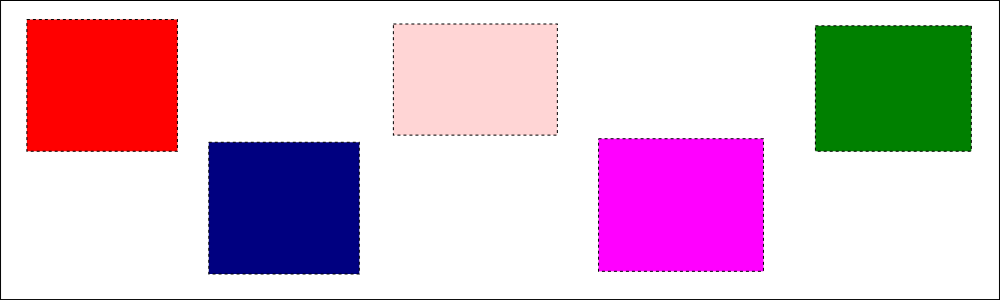
\includegraphics[width=0.9\textwidth]{figures/test_image}
            \caption{This is the caption of Sub-figure 12}
            \label{fig:subfig12}
        \end{subfigure}
    \caption{Two sub-figures}
\label{fig:sub-figures2}
\end{figure}

\subsection{Three figures together on a seperate page for floats}
Nulla at purus volutpat, accumsan arcu eget, commodo felis. Cras consequat
risus at rhoncus pellentesque. Aliquam tempor sodales purus in sodales. Sed ut
augue lobortis, mattis felis a, ultricies ante. Pellentesque ac tristique
ipsum, aliquet fermentum ipsum. Sed vel elit sed odio vestibulum semper id eget
enim. Nulla sed hendrerit tortor. Aliquam quam nisl, tempor ut nisl vel,
tristique facilisis libero. Suspendisse id rutrum ante. Duis sed luctus sapien.
Nullam sed quam justo.

\begin{figure}[p]
    \centering
    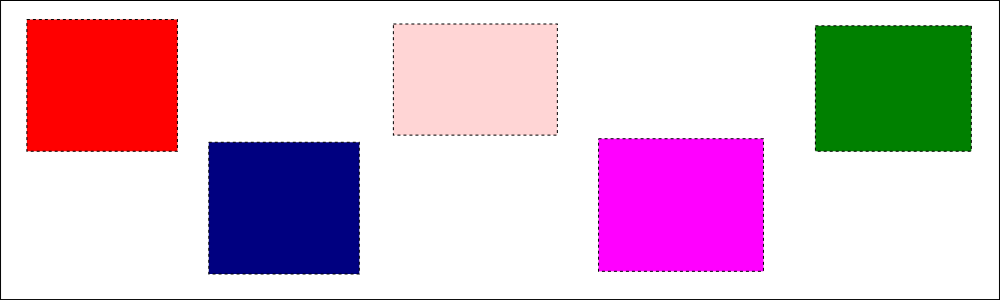
\includegraphics[width=\textwidth]{figures/test_image}
    \caption{Test Image 3}
    \label{fig:test_image3}
\end{figure}

\begin{figure}[p]
    \centering
    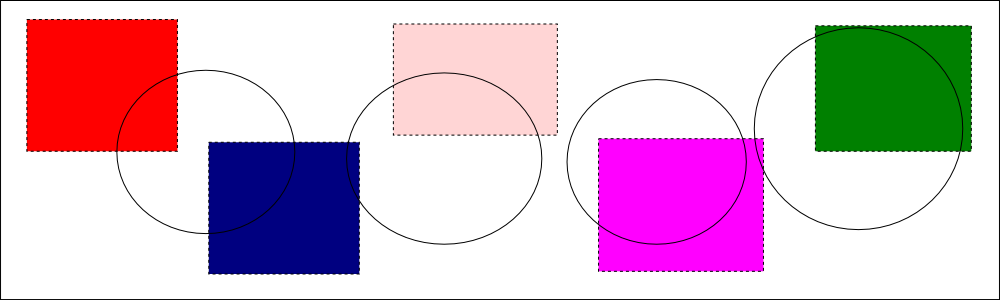
\includegraphics[width=\textwidth]{figures/test_image2}
    \caption{Test Image 4}
    \label{fig:test_image4}
\end{figure}

\begin{figure}[p]
    \centering
    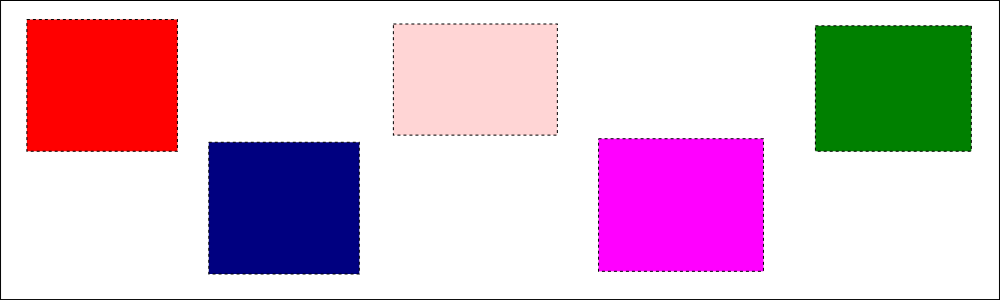
\includegraphics[width=\textwidth]{figures/test_image}
    \caption{Test Image 5}
    \label{fig:test_image5}
\end{figure}

% For more information about tables go to
% https://en.wikibooks.org/wiki/LaTeX/Tables
\section{Tables}
\subsection{One table}
Table \ref{tab:testtab2}, Aenean luctus quam ut neque viverra, quis vulputate
mi hendrerit. Nunc id leo id dui semper blandit. Nulla orci ligula, posuere non
lacinia non, aliquet non massa. Quisque gravida in mi eget volutpat. Fusce
convallis felis sed dolor ornare rhoncus. Nullam sed lacus id lectus venenatis
pulvinar eget ac arcu. Sed id turpis in leo sollicitudin euismod nec ac enim.
Nunc vitae lacus lectus.  Class aptent taciti sociosqu ad litora torquent per
conubia nostra, per inceptos himenaeos. Integer gravida, orci vitae viverra
ullamcorper, quam libero tempor est, non gravida magna eros id augue. In
lobortis et est auctor congue. Aliquam sed ante lacus. Vestibulum aliquam elit
eget elementum facilisis. Quisque eget felis eu leo pharetra pharetra.

\begin{table}[!ht]
  \centering
  \begin{tabular}{l*{6}{c}r}
      Team              & P & W & D & L & F  & A & Pts \\
      \hline
      Manchester United & 6 & 4 & 0 & 2 & 10 & 5 & 12  \\
      Celtic            & 6 & 3 & 0 & 3 &  8 & 9 &  9  \\
      Benfica           & 6 & 2 & 1 & 3 &  7 & 8 &  7  \\
      FC Copenhagen     & 6 & 2 & 1 & 3 &  5 & 8 &  7  \\
  \end{tabular}
  \caption{A floating test table.}
  \label{tab:testtab1}
\end{table}

\subsection{Two tables next to each other}
Some references to the tables on the next page, Table \ref{tab:testtab3} and
Table \ref{tab:testtab4} are sub-tables of Table \ref{tab:testtab2}. Aenean
luctus quam ut neque viverra, quis vulputate mi hendrerit. Nunc id leo id dui
semper blandit. Nulla orci ligula, posuere non lacinia non, aliquet non massa.
Quisque gravida in mi eget volutpat. Fusce convallis felis sed dolor ornare
rhoncus.

\begin{table}[!htb]
    \begin{subtable}{.5\linewidth}
      \centering
        \begin{tabular}{|r|l|}
            \hline
            7C0 & hexadecimal \\
            3700 & octal \\ \cline{2-2}
            11111000000 & binary \\
            \hline \hline
            1984 & decimal \\
            \hline
        \end{tabular}
        \caption{Caption for the first sub-table}
        \label{tab:testtab3}
    \end{subtable}%
    \begin{subtable}{.5\linewidth}
      \centering
        \begin{tabular}{|r|l|}
            \hline
            7C0 & hexadecimal \\
            3700 & octal \\ \cline{2-2}
            11111000000 & binary \\
            \hline \hline
            1984 & decimal \\
            \hline
        \end{tabular}
        \caption{Caption for the second sub-table}
        \label{tab:testtab4}
    \end{subtable}
    \caption{Caption for both tables}
    \label{tab:testtab2}
\end{table}

\subsection{One table with fixed column width}
Aenean luctus quam ut neque viverra, quis vulputate mi hendrerit. Nunc id leo
id dui semper blandit. Nulla orci ligula, posuere non lacinia non, aliquet non
massa. Quisque gravida in mi eget volutpat. Fusce convallis felis sed dolor
ornare rhoncus. Nullam sed lacus id lectus venenatis pulvinar eget ac arcu. Sed
id turpis in leo sollicitudin euismod nec ac enim. Nunc vitae lacus lectus.
Class aptent taciti sociosqu ad litora torquent per conubia nostra, per
inceptos himenaeos. Integer gravida, orci vitae viverra ullamcorper, quam
libero tempor est, non gravida magna eros id augue. In lobortis et est auctor
congue. Aliquam sed ante lacus. Vestibulum aliquam elit eget elementum
facilisis. Quisque eget felis eu leo pharetra pharetra.

\begin{table}[!ht]
  \centering
    \begin{tabular}{ | l | l | l | p{5cm} |}
    \hline
    Day & Min Temp & Max Temp & Summary \\ \hline
    Monday & 11C & 22C & A clear day with lots of sunshine.
    However, the strong breeze will bring down the temperatures. \\ \hline
    Tuesday & 9C & 19C & Cloudy with rain, across many northern regions. Clear spells
    across most of Scotland and Northern Ireland,
    but rain reaching the far northwest. \\ \hline
    Wednesday & 10C & 21C & Rain will still linger for the morning.
    Conditions will improve by early afternoon and continue
    throughout the evening. \\
    \hline
    \end{tabular}
  \caption{A floating test table with fixed column width.}
  \label{tab:testtab6}
\end{table}


\end{document}
